\documentclass{standalone}
\usepackage{pgfplots}
\pgfplotsset{compat=1.18}
\usepackage{xcolor}

% Define colors
\definecolor{impcolor}{RGB}{220,0,0}     % Red for IMP
\definecolor{synflowcolor}{RGB}{0,0,220} % Blue for SynFlow
\definecolor{snipcolor}{RGB}{0,150,0}    % Green for SNIP
\definecolor{unprunnedcolor}{RGB}{0,0,0} % Black for Unpruned

% Define styles for markers
\tikzset{
    marker/.style={mark size=3pt, thick},
    imp/.style={marker, color=impcolor, mark=triangle*},
    synflow/.style={marker, color=synflowcolor, mark=*},
    snip/.style={marker, color=snipcolor, mark=square*},
    unpruned/.style={thick, color=unprunnedcolor},
}

\begin{document}

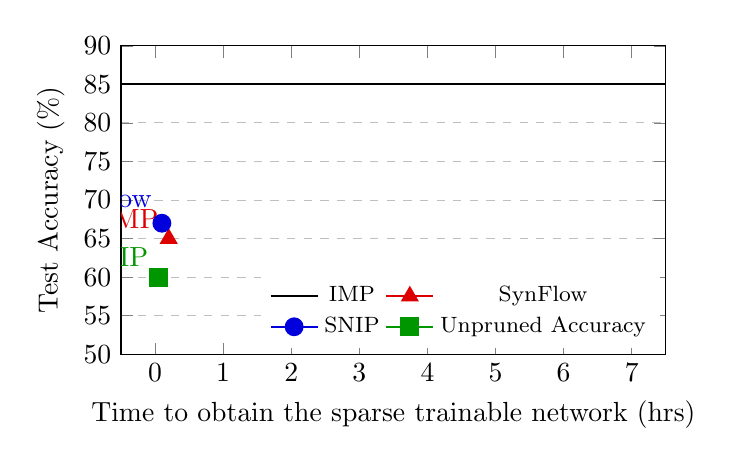
\begin{tikzpicture}
\begin{axis}[
    width=8.5cm,
    height=5.5cm,
    xlabel={Time to obtain the sparse trainable network (hrs)},
    ylabel={Test Accuracy (\%)},
    xmin=-0.5, xmax=7.5,
    ymin=50, ymax=90,
    ytick={50,55,60,65,70,75,80,85,90},
    xtick={0,1,2,3,4,5,6,7},
    ymajorgrids=true,
    grid style={dashed, gray!50},
    legend style={
        at={(0.99,0.02)}, 
        anchor=south east, 
        legend columns=2, 
        draw=none, % Remove border around legend
        fill=white, % Ensure white background
        font=\footnotesize % Smaller font for better fit
    },
]

% Unpruned accuracy line
\addplot[unpruned] coordinates {(-0.5,85) (7.5,85)} node[right,pos=0.99]{Unpruned Accuracy};

% IMP data point
\addplot[imp] coordinates {(0.2,65)} node[above left, pos=1]{IMP};

% SynFlow data point
\addplot[synflow] coordinates {(0.1,67)} node[above left, pos=1]{SynFlow};

% SNIP data point
\addplot[snip] coordinates {(0.05,60)} node[above left, pos=1]{SNIP};

% Add dummy plots for legend
\addplot[imp, draw=none] coordinates {(0,0)} \closedcycle;
\addplot[synflow, draw=none] coordinates {(0,0)} \closedcycle;
\addplot[snip, draw=none] coordinates {(0,0)} \closedcycle;

\legend{IMP, SynFlow, SNIP, Unpruned Accuracy}

\end{axis}
\end{tikzpicture}

\end{document}